\documentclass[a4paper]{article}
\usepackage[utf8]{inputenc}

\title{AAA Find Title!}
\author{Lorenzo Versini}
\date{December 2019}

%\usepackage{natbib}
%\usepackage{cite}
\usepackage[sorting=none]{biblatex}
\usepackage{float}
\bibliography{references}
\usepackage{graphicx}
\usepackage[most]{tcolorbox}
\usepackage{xcolor,sectsty}
\usepackage{multicol}
\setlength{\columnsep}{1cm}
\usepackage{bm}
\usepackage{makecell}
\usepackage{mathtools}
\usepackage{xcolor}

\usepackage{subcaption}
\hyphenation{op-tical net-works semi-conduc-tor am-pe-ro-me-ter de-mon-stra-te He-nce me-et a-ga-in spea-ches Chur-ches spee-ches}
\DeclarePairedDelimiter\abs{\lvert}{\rvert}%
%\usepackage[width=14cm, left=2cm]{geometry}
\usepackage[width=15cm]{geometry}

\definecolor{astral}{RGB}{46,116,181}
\subsectionfont{\color{astral}}
\sectionfont{\color{astral}}

\tcbset{enhanced,colback=astral!5!white, boxrule=0.4pt,sharp corners, colframe=astral!75!black,fonttitle=\bfseries}

\begin{document}


\begin{titlepage}
	\begin{center}
		\vspace*{1cm}
		
        \Huge
        \textbf{\color{astral}Article Title}
        
        \LARGE
        \vspace{0.5cm}
        \color{astral}{Article Subtitle}
        \color{black}
        \vspace{1.5cm}
        
        \textbf{Lorenzo Versini}
        
        
        \vfill
        Wordcount:  
        
        \Large
        Physics\\
        Imperial College London\\
        Date
        
	\end{center}
\end{titlepage}
\twocolumn
%\begin{multicols}{2}
\section{Introduction}


Whisper in an open green field outdoors and nobody will hear you. Whisper in St. Paul Whispering Gallery (London) and people at 30m distance will be able to listen to you.

It is clear that the way we perceive sound and hence a good part of how we live the world, is affected by the surrounding and the particular geometry of the place where we interact.

Understanding of how sound is modified by the environment, can lead to a better exploitation of architectural spaces architects which can therefore be optimized to suit specific functions as can be a concert or a religious rite.

Therefore, a question we want to dig into is: how do exactly closed spaces ``amplify" sounds? What properties of sound make a particular concert hall sound good? Can we even objectively say what is good and what is not?

The answer to the last question is a yes and no. Acoustic has much to do with human taste which is unsurprisingly subjective. 

However, general preference patterns can be evaluated within societies and cultures and by understanding the connection between them and the physics of what is objectively measured, powerful tools for acoustic architects can be created.

\section{Pressure waves and whispering on Walls}

We will start with the very basic, by introducing sound waves. A sound wave is a pressure fluctuation in air \cite{book:university_physics} which travels in the medium with a speed $c$ in the order of 340 m/s and it is described by the wave equation,

\begin{equation}
\frac{\partial^2 u}{\partial t^2} = c^2 \frac{\partial^2 u}{\partial x^2}
\end{equation}

When a sound wave hits a surface it is partly absorbed and partly reflected, as a light wave on domestic mirror would do.

Sometimes, it is useful and valid to think at sound waves in terms of rays departing from a source and reflecting on surfaces. This is not completely obvious, as we generally deal with bigger wavelength than light (e.g. the A note Orchestras tune on, has a wavelength of approx. 0.8m).

We all have the intuitive understanding that the further we go, the weaker the wave is: listening someone speaking far from us is hard if we are in the middle of nowhere surrounded by nothing.

Indeed, similarly to the light from a star, sound waves follow a
\begin{equation}
\frac{1}{r^2}
\end{equation}

law, which means that if we double the distance, the amplitude of the pressure oscillation reduces by four.

By carefully shaping the geometry of a closed environment, these properties of sound waves can be exploited to generate peculiar effects!

An example is the Whispering gallery situated in St. Paul Cathedral (London) which is famous for the fact that if two people stand at opposite sides of the room along the wall, they can whisper each other and still listening what they are saying \cite{article:whispering}.

\begin{figure}
\centering
\begin{tcolorbox}[drop lifted shadow]


\includegraphics[scale=0.28]{rayleigh_experiment}
\caption{ Shows the experiment Rayleigh performed. A singing bird was firstly placed in front of a flicking candle at 2m and no movement in the flame could be seen. Then the bird and the candle were placed inside a cylindrical metallic plate and the flame moved as the animal sang. Lastly, an obturating screen was placed along the metallic plate and the absence of movement in the flame showed that sound waves were propagating along the surface of the screen }
\label{fig:duck}

\end{tcolorbox}\par\bigskip
\end{figure}

An explanation to this surprising phenomenon was proposed by Lord Rayleigh in 1896 and it turned out to agree with numerical and physical tests \cite{article:whispering}. 

His idea was that surface sound waves would reflect and propagate along the the walls, finally reaching the person on the other side.

He performed a simple experiment to demonstrate his hypothesis. He placed a bird and a flame at a distance of 2m one from the other and noticed that when the bird sang, no flickering in the flame could be noticed \cite{article:whispering}.\\
Then he placed bird and flame in a cylindrical metallic plate of diameter of 2 meters at the same distance and noticed that as the bird sang, the flame started to fickle.\\
Lastly, he used an obturating screen to obstruct the way along the inner side of the metallic surface and he noticed that this time the flame did not fickle. \cite{article:whispering}

This enforced the idea that because of the circular geometry, sound waves propagated along the surface of the walls, allowing less energy losses and thus explaining the peculiarities of architectural structures.

\section{Interpreting Judgments}
If you ask a professional musician to play in a room and then to judge the quality of the acoustic, he will come out with some bizarre words like \textit{dry}, or \textit{full}.

Then, if you ask another musician, there is a good chance that he will independently agree with the other’s opinion. Therefore, there must be some physical effect, something which makes a room’s sound dry.

However, in order to find that, we need to understand what dry scientifically means! 

This was done by comparing people’s judgments with room’s measured parameters for a variety of different architectural spaces.

This leaded to a bridge between subjective parameters that we use in our everyday lives and objective and mathematical parameters which can be used to design and characterise acoustic spaces. [3]

There are many parameters, however here we will just meet two: \textit{reverberance} and \textit{clarity}.

\section{Reverberance}
A main parameter is reverberance. The word comes from the prefix “re-” which means again and the latin “verberare” i.e. to whip [4]. 
\\
\begin{tcolorbox}[drop lifted shadow, rounded corners]
\textit{Reverberance: the quality of a sound that lasts for long after the source is shut. \cite{book:acoustic3}}
\end{tcolorbox}\par\bigskip
What causes a sound to last in a room even if the sound source has been shut?

\begin{figure}
\centering
\begin{tcolorbox}[drop lifted shadow]

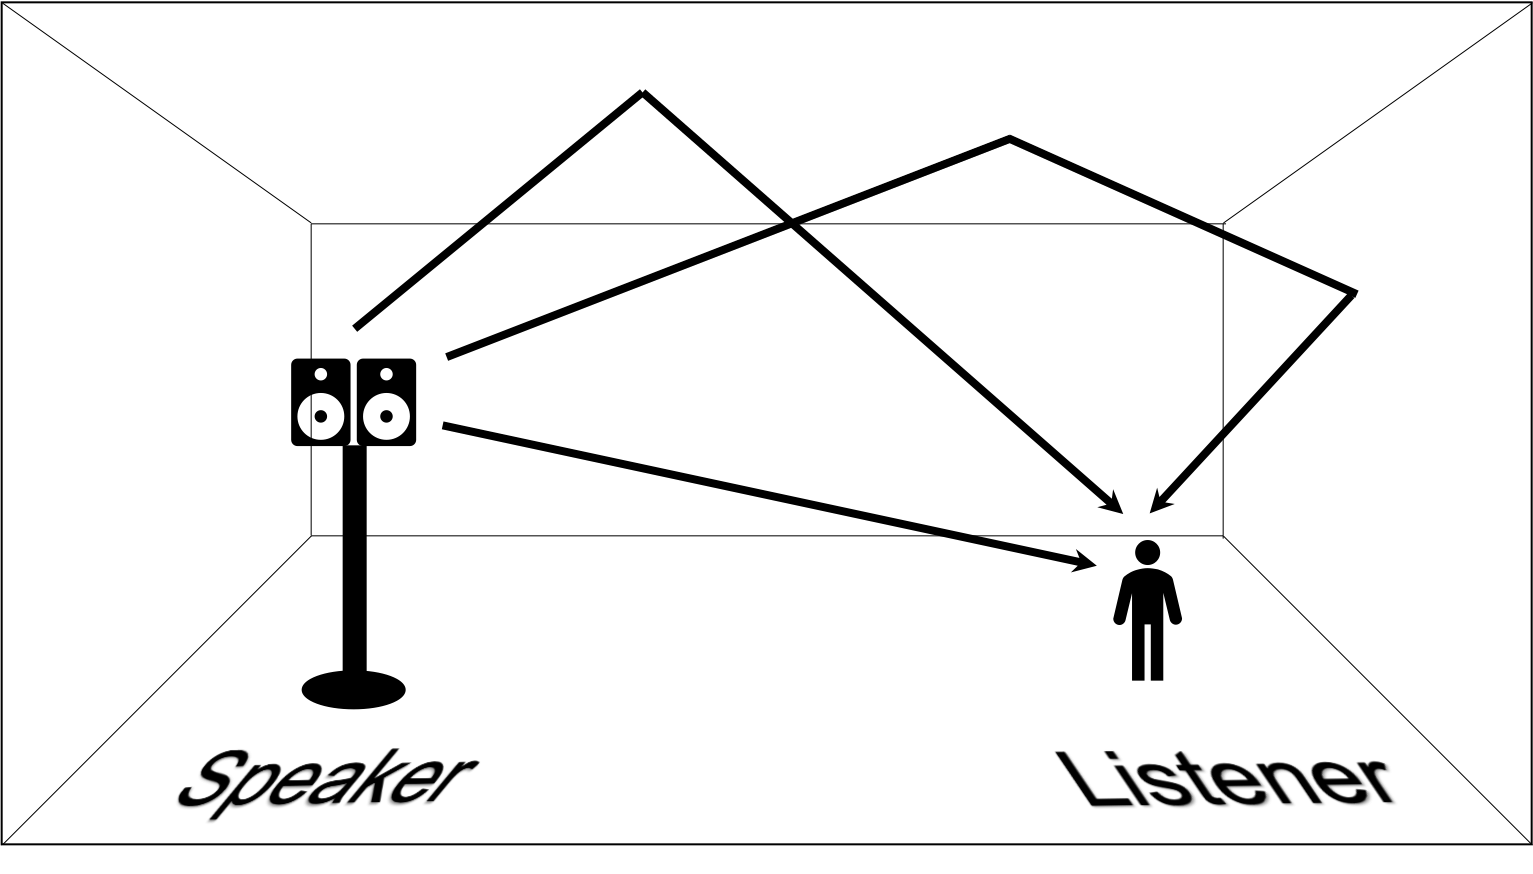
\includegraphics[scale=0.22]{reverberant-box}
\caption{Schematic representation of a room. Sound from the speaker reaches the listener at different times, causing the sound level to increase over time}
\label{fig:box}

\end{tcolorbox}\par\bigskip
\end{figure}

Let's analyse the scenario represented in Fig. \ref{fig:box}, where a speaker produces a sound in a room and there is a listener. Firstly, he is reached by the direct sound (ray \textbf{A}), then all the other reflections reach him at following times (i.e. \textbf{B}, \textbf{C}).

Therefore, the sound level as perceived by the listener increases over time. Eventually, an equilibrium is reached between the speaker continuing adding energy as sound waves and the absorption of air and surfaces (e.g. walls) and a constant intensity is reached.

Similarly, as the source is suddenly shut, the intensity level takes time to decrease, as all the energy stored as sound waves needs to be absorbed or dispersed. 

This process requires time according to the absorption coefficients of the surfaces in the room. If the sound stays for long, then we say that the room is reverberant.

Hence, it seems natural that a way to characterise the reverberance of a closed space, we could measure how long a sound stays a room after the source was shut.

The actual definition of the \textit{reverberation time} involves the intensity of a sound $L_I$ i.e. the logarithm,

\begin{equation}
L_I = 10 \log_{10}{\frac{I}{I_0}}\ \mathrm{dB}
\end{equation}

where $I_0$ is a reference value and it is the lowest intensity that an average person can perceive at $1000\ \mathrm{Hz}$ \cite{book:acoustic2}.

Then, the reverberation time is defined as the time that it takes to the sound in a room to decrease by $60$ decibels after shutting down the source. In practice, the drop time is evaluated between $-5 \mathrm{dB}$ and $-35 \mathrm{dB}$ as follows,

\begin{equation}
T = 60 \mathrm{dB} \frac{t_{-35} - t_{-5}}{(-5\mathrm{dB}) - (-35\mathrm{dB})}
\end{equation}

Two good reasons why the reverberation time is evaluated according to a logarithmic scale rather than a linear one are that the intensity level is a scale which better approximates the way we perceive sound \cite{book:acoustic2} and that we expect the intensity fall to be exponential-like \cite{book:acoustic} and exponential relations appear as linear in a logarithmic scale.

\subsection{Absorption and Reverberation Time\label{sub:absorption}}

In $1988$ Sabine was called to solve an issue with the \textit{Fogg Art Museum} lecture hall in Harvard. Sound in the room persisted for over $5$ seconds, therefore making extremely hard for people to understand speeches.

By adding $550$ thick cushions to the room, Sabine achieved reducing that time to about 1 second \cite[p. ~300]{book:acoustic2}.

We saw in previous section that sound energy introduced by a speaker in a room does not increase indefinitely. This is due to absorption and dissipation due to cushions, walls, air and even people! Indeed, an empty concert hall sounds differently than a filled one.


Then, it is not hard to imagine that the more absorptive is a room, the fastest the sound level decreases as the source is shut and therefore the less reverberating the room is.

There exist an equation which relates the reverberation time of a room which its characteristics and it is called \textit{Sabine equation}. It was developed by Wallace Clement Sabine  who was an American acoustic pioneer \cite[p. ~316]{book:acoustic}. 



\begin{equation}
T = \frac{0.161 V}{S \alpha^* + 4 m V}
\end{equation}
where:
\begin{itemize}
\item $A$ and $V$ are respectively total surface and volume of the room;
\item 0.161 is an empirical factor;
\item $\alpha^*$ is the surface-weighted sum of the sound absorption coefficients $\alpha_i$ and it is defined as $a^* = \frac{1}{S}\sum_i{\alpha_i S_i}$;
\item $m$ is a correction factor added in a second moment which takes in a account air absorption.
\end{itemize}


Table \ref{table:material} lists some absorption coefficients for multiple materials at a frequency of $1\mathrm{kHz}$ \cite{site:acoustic_absorption}.




\begin{table}
\caption{}
\begin{tabular}{ |c|c| } 
 \hline
 \textbf{material} & $\bm{\alpha\  [\mathrm{sabin}]}$\\ 
 \hline\hline
 Walls, rendered brickwork & $0.03$\\ 
 \hline
 Marble floor & $0.02$\\ 
 \hline
 \makecell{Curtains (0.2 kg/m2) hung \\ 90 mm from wall} & $0.63$\\
 \hline
 \makecell{Audience on wooden\\ chairs, 1 per m2} & $0.69$ \\
 \hline
\end{tabular}
\label{table:material}
\end{table}

\section{Speeches and Music}
A question we might ask ourselves is what a generally good reverberation time is for a certain type of room.

The answer is that it depends and there is is much disagreement on the choice of the reverberation time and other parameters. This is because they depend on the purpose of the room, on personal taste and even on cultural traditions.

However, some general features can be found. Dealing with general purposes, speeches have different requirements than music. A high reverberation time could undermine the intelligibility of a person speaking because load vowels would cover consonants resulting in a blurred effect.

On the other hand, a \textit{dead space} (i.e. where reverberance is very low) can be unpleasant for music \cite{book:acoustic3} as the dry acoustic decreases loudness and makes harder for an orchestra to have a more compact and unite sound. 

Therefore, we can make a first distinction: spaces designed for music will have different characteristics than the ones designed for speeches.

However, inside these two macro functions, there are still sensible differences! Rock music has different requirements than classic one. Churches are very peculiar for they host both speeches and music. Therefore, they need to find a compromises between their parameters.

\subsection{A good Concert Hall}
Generally, Concert Halls have reverberation times in the order of $1.5 - 2.2$ seconds.

However, we anticipated that different types of music require different acoustics. For instance, Baroque music would sound best with values in the order of $1.5-1.7$ seconds, whereas Romantic music would require a slightly higher reverberation time.

Although there are these differences, some common characteristics can be outlined \cite{book:acoustic3}.

\subsubsection*{Clarity}
It is unpleasant for a room to be heavily reverberating. Think of a violinist executing a fast piece: if reverberance is too high, then the effect would be the one of a blurred sequence of notes.

Instead, we want to hear notes neatly and \textit{clearly}.
\\
\begin{tcolorbox}[drop lifted shadow, rounded corners]
\textit{Clarity: The degree to which rapidly occurring individual sounds are distinguishable \cite{book:acoustic3}}
\end{tcolorbox}\par\bigskip

When reflections arrive within $80 \mathrm{ms}$
from the direct sound, our ear integrates their contributions and we perceive them as a single amplified sound \cite{book:acoustic}.

Hence, the blurred effect is given by reflections arriving later than this time window. The stronger, the more noticeable they are. 

Hence, a reasonable way to quantify clarity ($C_{80}$) is comparing sound contributions within the first $80$ milliseconds with all the other reflections.

\begin{equation}
C_{80} = 10\log{\frac{\int_0^{80ms}{I_{(t)}dt}}{\int_{80ms}^{\infty}{I_{(t)} dt}}} \mathrm{dB},
\end{equation}
where $I_{(t)}$ is the sound intensity which is integrated over time to model the total perceived effect.

We can give a look to \textit{Santa Cecilia} Concert Hall in Rome designed by Renzo Piano as an example.

Fig. \ref{fig:clarity} shows the values of clarity measured in front of the stage at multiple frequencies. We can see that more energy is in the tail of sounds for low frequencies whereas there is greater clarity for higher frequencies.

An optimal values for medium frequencies ($500-1000\ \mathrm{Hz}$) is 0 \cite{article:santa_cecilia_acoustic} and we can see from the plot that the hall is quite close to that.

\begin{figure}
\centering
\begin{tcolorbox}[drop lifted shadow]

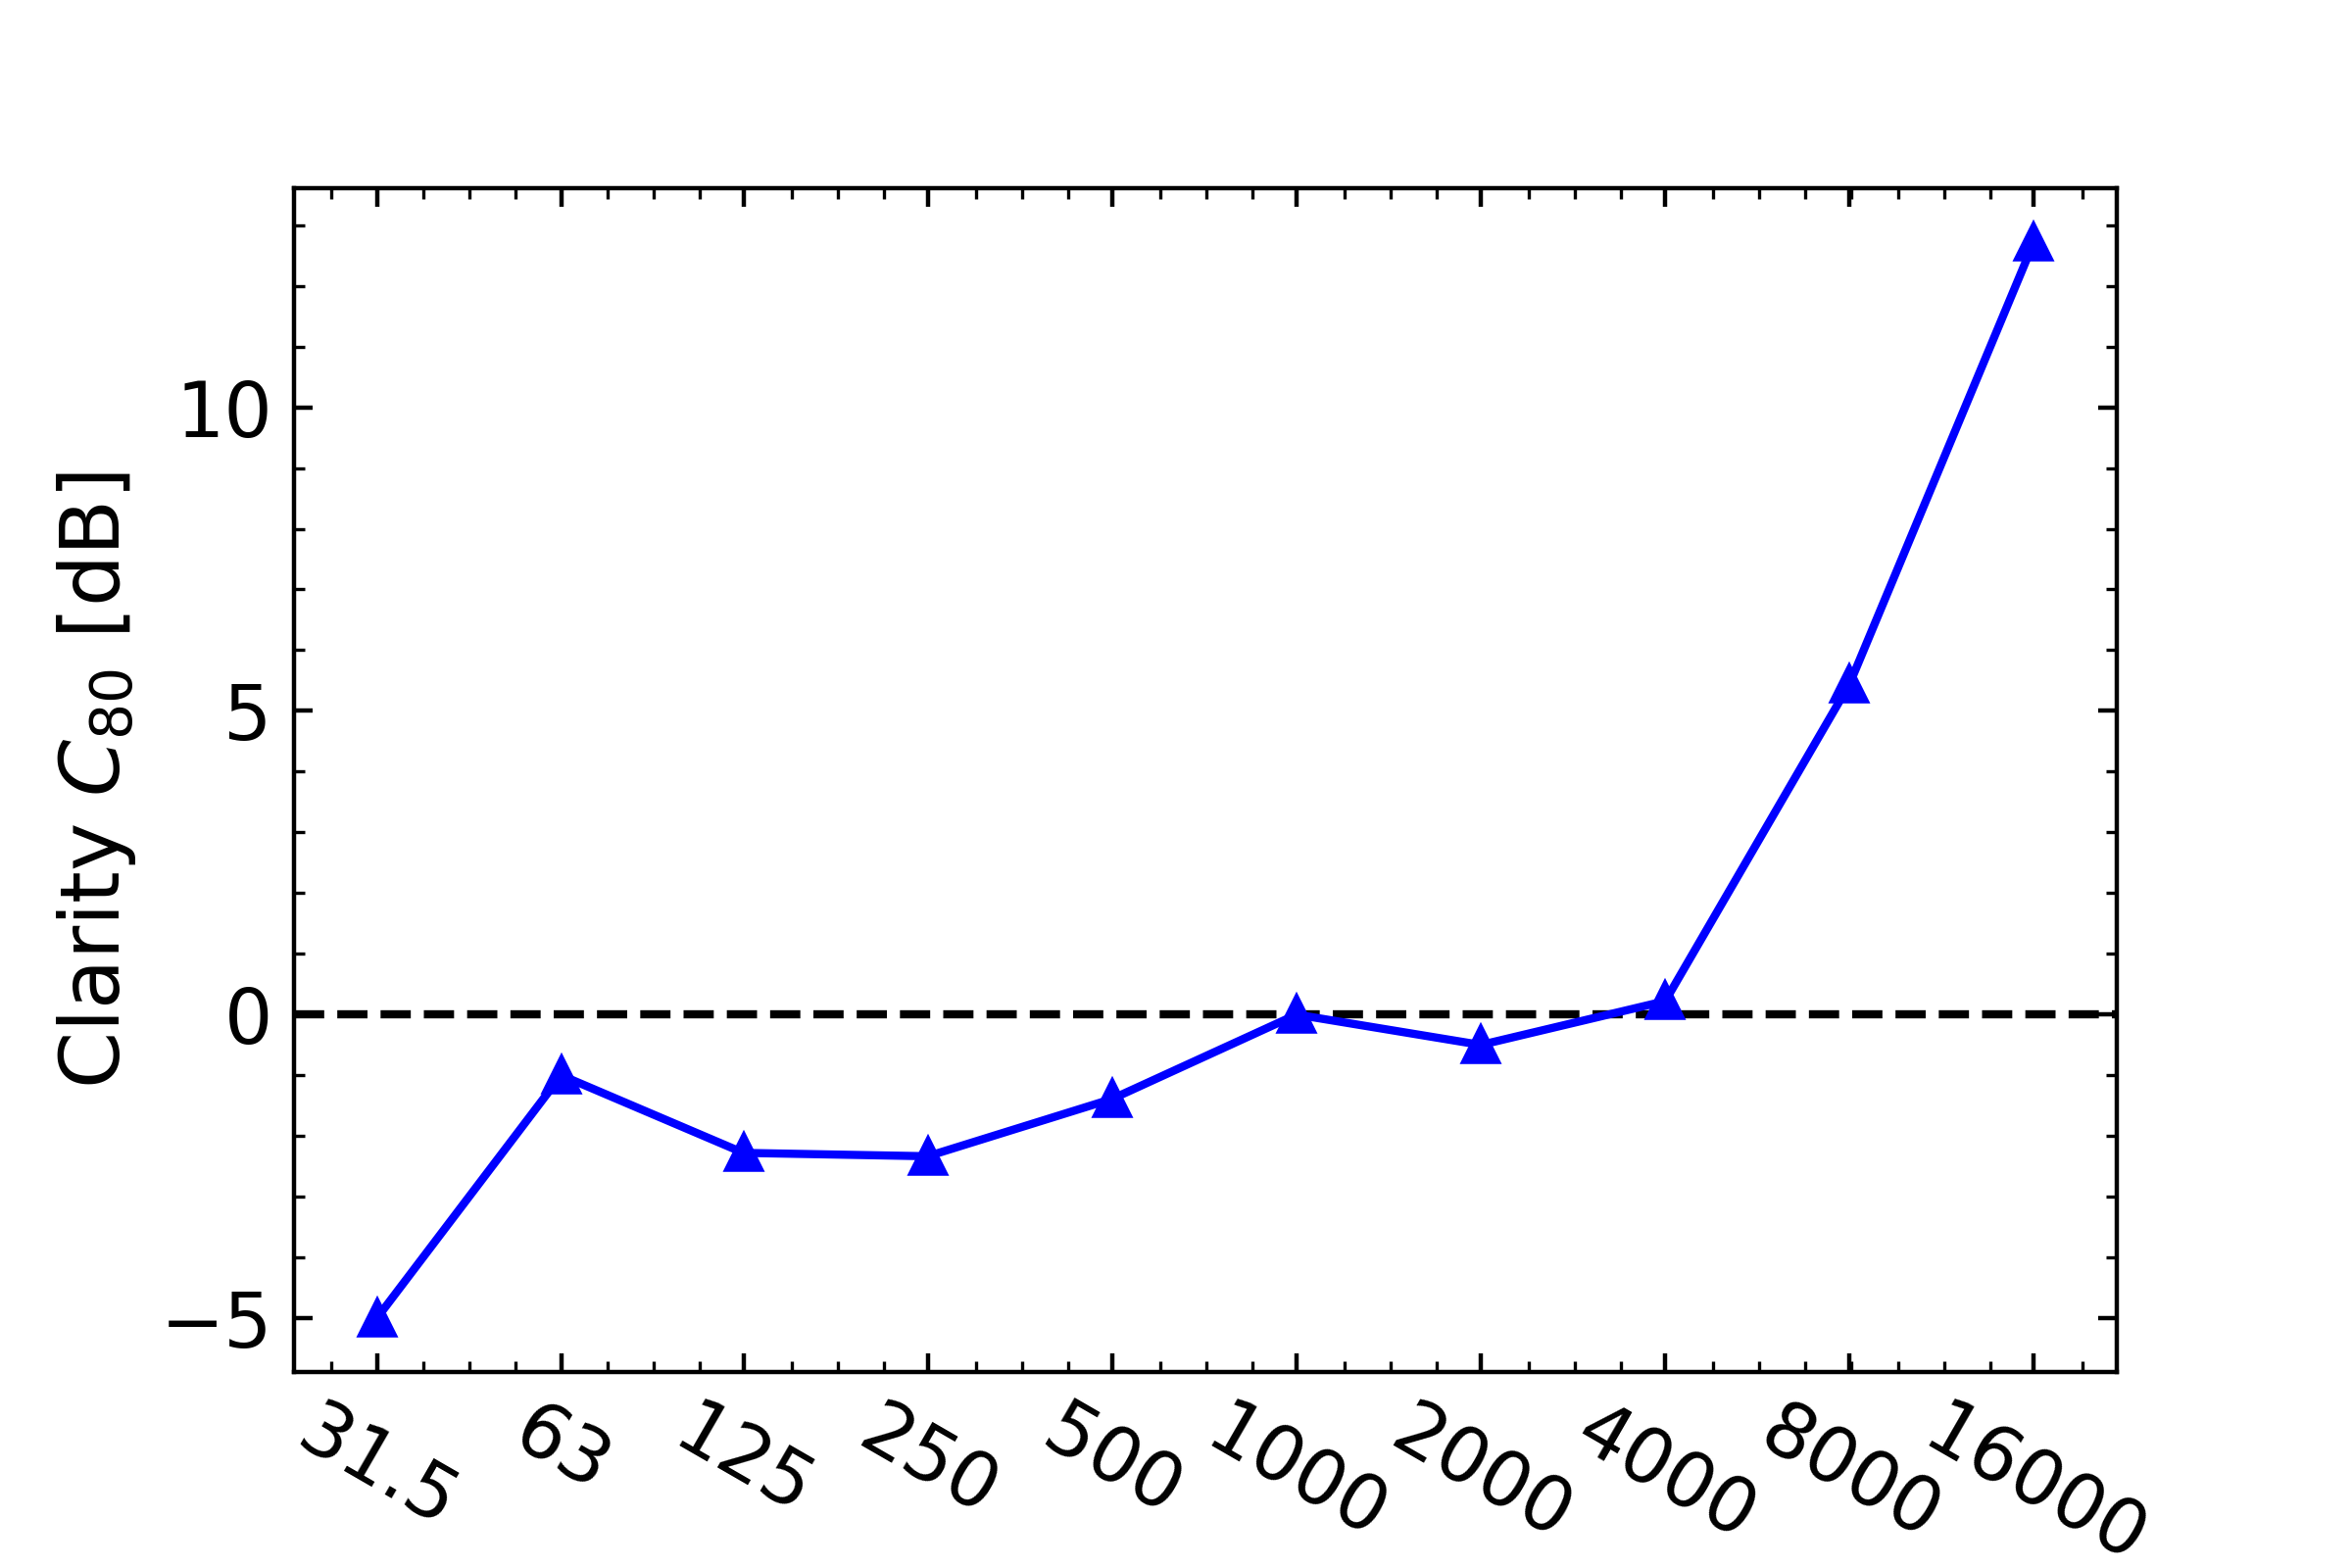
\includegraphics[width=6cm]{graph}
\caption{.. Elaborated from \cite{article:santa_cecilia_acoustic}}
\label{fig:clarity}

\end{tcolorbox}\par\bigskip
\end{figure}

\subsubsection*{Spaciousness}

People usually say that watching movies home is great, but cinemas are far better.

Well, one difference can be spot in the quality of the sound experience. At home we usually have a television with an integrated speaker. Sound is stereo, but it comes just from one direction.

On the other hand, in cinemas we are usually surrounded by a set of speakers, each one with its function. The result is that we feel \textit{inside} the sound, surrounded by it.

This sensation is important for a concert hall and it is called \textit{spaciousness}.\\


\begin{tcolorbox}[drop lifted shadow, rounded corners]
\textit{Spaciousness: The feeling of sound arriving from many different directions in contrast to a mono-phonic impression of all sound reaching the listener through a narrow opening \cite{book:acoustic}}
\end{tcolorbox}\par\bigskip

It has been found experimentally that this factor depends on the strength of lateral reflections. One of the aspects which contribute to spaciousness is the \textit{apparent source width} ($ASW$), which is the impression we have of the source being wider than what it actually is \cite{book:acoustic}.

A parameter which experimentally describes $ASW$ and which is related to people's sound preferences is the \textit{interaural cross-correlation} ($IACC$).

This is a sort of comparison between the sound pressure ($h_{(t)}$) registered with a microphone which has two openings in opposite direction and which can therefore measure a signal coming from the right of the room ($h_{R(t)}$) and one from the left ($h_{L(t)}$).

Surprisingly, our body too has a similar microphone and it is called ears.

\begin{equation}\label{eq:iacc}
IACC_{t_1, t_2} = \mathrm{max}\abs*{\frac{\int_{t_1}^{t_2}{h_{L(t)}h_{R(t+\tau)}dt}}{\sqrt{\int_{t_1}^{t_2}{h^2_{L(t)}dt \int_{t_1}^{t_2}{h^2_{R(t)}dt}}}}}
\end{equation}

$\tau$ is a value which is changed to maximise the ratio and takes in account for the signal phase shift due to the ear's distance. Therefore, it takes values within $\pm 1\mathrm{ms}$ which is about the time that takes to sound to travels from one ear to the other.

The interval $t_1$ and $t_2$ for the $ASW$  is taken to be $(t_1, t_2) = (0\mathrm{ms}, 100\mathrm{ms})$. We can see from eq. (\ref{eq:iacc}) that if $h_{L}(t)=h_{R}(t + \tau_{shift})$, then the value of $IACC$ is $1$.

However if they differ (e.g. because of reflections), then $IACC$ will take values between $0$ and $1$ and the smaller it is, the greater is the sensation of spaciousness \cite{book:acoustic}.

As an example, Santa Cecilia Hall has an $IACC$ between $0.4$ and $0.6$ which is a good range \cite{article:santa_cecilia_acoustic}.

\subsection{Acoustic in churches }
Previously, we said that culture affects the definition of a good reverberance. A gazing example is the way reverberation time in churches changed during time.

The origin of Christian worshipping buildings has its roots in jew synagogues. They were used for rituals (sermon centered) and community meetings and the acoustic properties were adapted to favour speech and group singing \cite{article:acoustic:churches}. 

Around  $315$ CE, emperor Constantine recognized Christian churches as official. Let free to publicly practice their religion, Christians started adapting Roman basilicas model to their religious buildings. These were characterised by high roofs leaded to  extremely high resonance times.

An example is St. Paolo Fuori dalle Mura in Rome ($386$ CE) which has a reverberation time of 9.1 seconds. This is extremely high even if compared with a symphonic concert hall as the great hall of \textit{Academia Nazionale di Santa Cecilia} which has a reverberation time of $2.2$ seconds.

It has been speculated \cite{article:acoustic:churches} \cite{article:acoustic:history} that these acoustic characteristics caused  main changes in the liturgy which became more and more centered on music and less on spoken parts.

\begin{figure}[H]
\centering
\begin{tcolorbox}[drop lifted shadow]
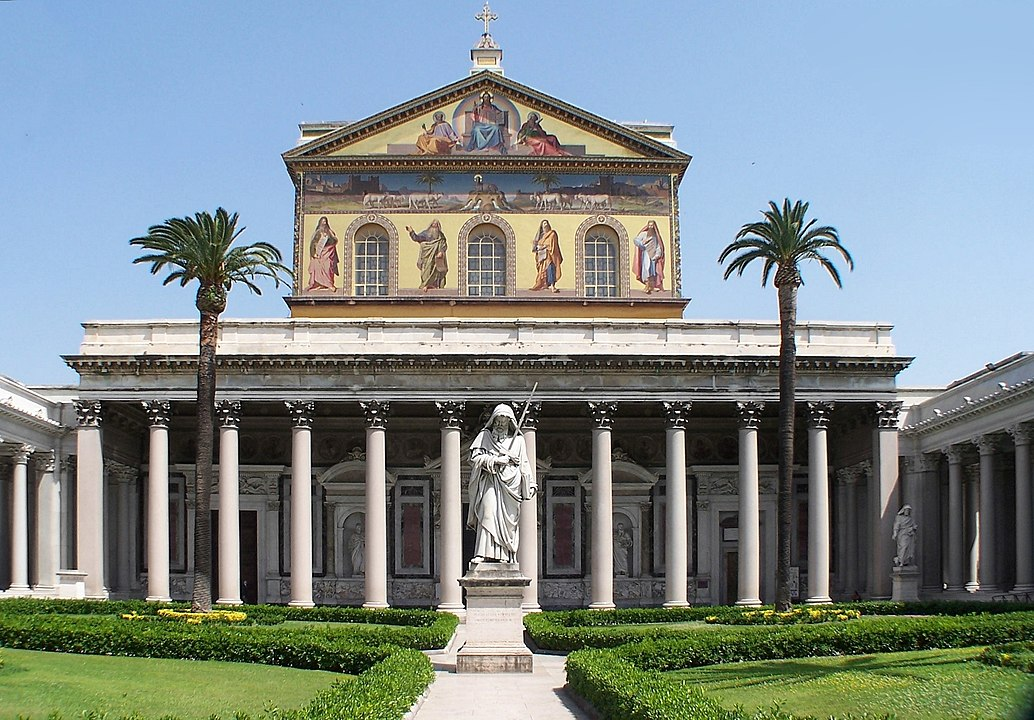
\includegraphics[scale=0.16]{san-paolo}
\caption{[from Wikipedia]}
\label{fig:san-paolo}
\end{tcolorbox}\par\bigskip
\end{figure}

Indeed, Gregorian chants with their long and sustained sounds well matched the characteristics of the basilicas: singing every syllable on a different pitch helped with the intelligibility of words otherwise compromised by a \textit{blurred} effect.

Liturgy continued evolving and polyphony started being practiced. At the beginning the new melodies added to the chant had only a sustaining function however, this practice kept getting more and more sophisticated. 

Eventually, an overlapping of several melodies and texts made almost impossible for the listener understanding the words \cite{article:acoustic:churches} \cite{book:history_music}. Moreover, most of them would have been inaccessible anyways because Latin was not understood by common people.

The architectures of these new changes were Gothic Churches, characterised by high roofs and large reverberation times.

Salisbury Cathedral, completed in 1258, had a reverberation time of 6 seconds. Nowadays, a system of loudspeakers and other tools is used to solve issue of speech intelligibility \cite{site:salisbury:reverberation}.

With Reformation, the attention was brought back on texts and audience participation. For instance, vernacular was used instead of Latin so that ordinary people could understand what was said. On the architecture point of view, acoustic was made drier and there was a general attempt of reducing reverberation time.

Thomaskirche in Leipzig used wooden panelling and hanging draperies to increase sound absorption (recall Sec. \ref{sub:absorption}) achieving a reverberation time of $1.6$ when fully occupied \cite{article:acoustic:churches}.




\printbibliography

%\bibliographystyle{plain}
%\bibliography{IEEEabrv,references}


%\end{multicols}

\end{document}
